%%%%%%%%%%%%%%%%%%%%%%%%%%%%%%%%%%%%%%%%%
% Beamer Presentation
% LaTeX Template
% Version 1.0 (10/11/12)
%
% This template has been downloaded from:
% http://www.LaTeXTemplates.com
%
% License:
% CC BY-NC-SA 3.0 (http://creativecommons.org/licenses/by-nc-sa/3.0/)
%
%%%%%%%%%%%%%%%%%%%%%%%%%%%%%%%%%%%%%%%%%

%----------------------------------------------------------------------------------------
%	PACKAGES AND THEMES
%----------------------------------------------------------------------------------------

\documentclass{beamer}

\mode<presentation> {

% The Beamer class comes with a number of default slide themes
% which change the colors and layouts of slides. Below this is a list
% of all the themes, uncomment each in turn to see what they look like.

%\usetheme{default}
%\usetheme{AnnArbor}
%\usetheme{Antibes}
%\usetheme{Bergen}
%\usetheme{Berkeley}
%\usetheme{Berlin}
%\usetheme{Boadilla}
%\usetheme{CambridgeUS}
%\usetheme{Copenhagen}
%\usetheme{Darmstadt}
%\usetheme{Dresden}
%\usetheme{Frankfurt}
%\usetheme{Goettingen}
%\usetheme{Hannover}
%\usetheme{Ilmenau}
%\usetheme{JuanLesPins}
%\usetheme{Luebeck}
\usetheme{Madrid}
%\usetheme{Malmoe}
%\usetheme{Marburg}
%\usetheme{Montpellier}
%\usetheme{PaloAlto}
%\usetheme{Pittsburgh}
%\usetheme{Rochester}
%\usetheme{Singapore}
%\usetheme{Szeged}
%\usetheme{Warsaw}

% As well as themes, the Beamer class has a number of color themes
% for any slide theme. Uncomment each of these in turn to see how it
% changes the colors of your current slide theme.

%\usecolortheme{albatross}
%\usecolortheme{beaver}
%\usecolortheme{beetle}
%\usecolortheme{crane}
%\usecolortheme{dolphin}
%\usecolortheme{dove}
%\usecolortheme{fly}
%\usecolortheme{lily}
%\usecolortheme{orchid}
%\usecolortheme{rose}
%\usecolortheme{seagull}
%\usecolortheme{seahorse}
%\usecolortheme{whale}
%\usecolortheme{wolverine}

%\setbeamertemplate{footline} % To remove the footer line in all slides uncomment this line
\setbeamertemplate{footline}[page number] % To replace the footer line in all slides with a simple slide count uncomment this line

%\setbeamertemplate{navigation symbols}{} % To remove the navigation symbols from the bottom of all slides uncomment this line
}

\usepackage{graphicx} % Allows including images
\usepackage{booktabs} % Allows the use of \toprule, \midrule and \bottomrule in tables
\usepackage{xcolor}% or package color
\usepackage{amssymb}
\usepackage{amsmath}
\usepackage{bm}
\usepackage{mathtools}
\usepackage{tikz}
\usetikzlibrary{trees}

\graphicspath{{./Figures/}}

%----------------------------------------------------------------------------------------
%	TITLE PAGE
%----------------------------------------------------------------------------------------

\title[lab meeting]{Evolutionary rescue by introgressive hybridization} % The short title appears at the bottom of every slide, the full title is only on the title page

\author{F.J.H. de Haas \& S.P. Otto} % Your name

\date{\today} % Date, can be changed to a custom date

\begin{document}

\begin{frame}
\titlepage % Print the title page as the first slide
\end{frame}

\begin{frame}{Orr and Unckles 2014}

Evolutionary rescue is characterized by a U-shaped curve of population size.

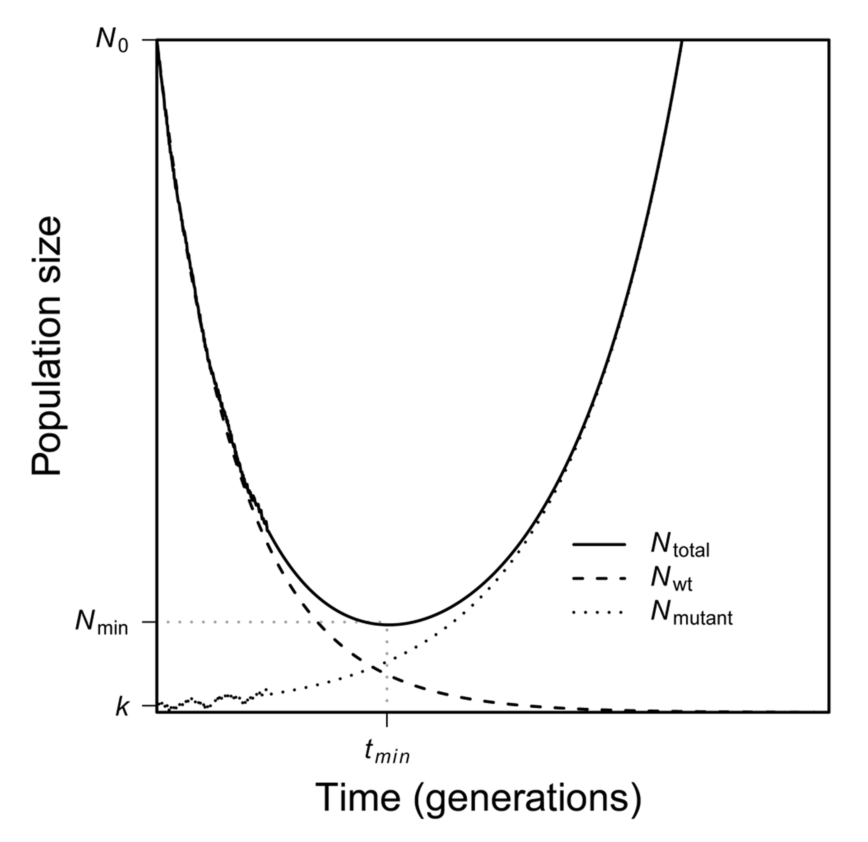
\includegraphics[width=0.5\columnwidth]{Ushape_ER.png}

\end{frame}

\begin{frame}{Analytical model}

\begin{equation}
    \begin{array}{l}
	F_w[t+1] = \overbrace{\frac{1}{2} (F_w[t]+F_b[t]) p_b[t+1]}^\text{$w$ x $b$}  + \overbrace{F_w[t] (1-p_b[t+1])}^\text{$w$ x $w$}
	 \\ \\
	F_b[t+1]  = \overbrace{\frac{1}{2} (F_w[t]+F_b[t]) (1-p_b[t+1])}^\text{$b$ x $w$} 
	+ \overbrace{F_b[t] p_b[t+1]}^\text{$b$ x $b$}
	\end{array}
\end{equation}

Assumptions: \\
1) Infinite population size \\
2) Infinite \# of loci \\
3) Free recombining loci ($r = 0.5$) 
    
\end{frame}

\begin{frame}{Model}
    \begin{equation}
    F_b[t] = \sum_{i=1}^t 2^{-i} (1-p_b[i])
\end{equation}
\end{frame}


\begin{frame}{Discrete Markov Model}
\footnotesize

$\bold{P} = \{\{G_{AB},G_{Ab},G_{aB},G_{ab}\}\} \text{ such that } G_i\in\{0,1,...,n\}$\\ 
$\bold{X},\bold{Y} \in \bold{P}$. \\

Probability of going from $\bold{X}$ to $\bold{Y}$
\begin{equation*}
\bold{M}_{\bold{Y},\bold{X}}=
\begin{aligned}
\begin{cases}
\begin{cases}
    b_{AB}, & \text{if } \bold{Y} = \bold{X} + \{1,0,0,0\}; \\
    b_{Ab}, & \text{if } \bold{Y} = \bold{X} + \{0,1,0,0\};  \\
    b_{aB}, & \text{if } \bold{Y} = \bold{X} + \{0,0,1,0\}; \\
    b_{ab}, & \text{if } \bold{Y} = \bold{X} + \{0,0,0,1\}; \\
    d_{AB}, & \text{if } \bold{Y} = \bold{X} + \{-1,0,0,0\}; \\
    d_{Ab}, & \text{if } \bold{Y} = \bold{X} + \{0,-1,0,0\};  \\
    d_{aB}, & \text{if } \bold{Y} = \bold{X} + \{0,0,-1,0\}; \\
    d_{ab}, & \text{if } \bold{Y} = \bold{X} + \{0,0,0,-1\}; \\
    1, & \text{if}\ \bold{X} = \bold{Y} = \{0,0,0,0\}; \\
    0, & otherwise;
\end{cases}  & \text{for}\ \bold{X}_1, \bold{X}_2 \neq n; \\
\begin{cases} 
    1, & \text{if}\ \bold{X}_1 = \bold{Y}_1 = n; \\
    1, & \text{if}\ \bold{X}_2 = \bold{Y}_2 = n;  \\
    \mathrlap{0,}\hphantom{d_{AB},} & otherwise;
\end{cases} & otherwise;
\end{cases},
\end{aligned}
\end{equation*}
where $C$ is a normalization constant.
\normalsize

\end{frame}

\begin{frame}{Probabilites of birth-death model}

    $b_{AB}-d_{AB} = b_{Ab}-d_{Ab}=(W_A-1)$ \& $b_{aB}-d_{aB} = b_{ab}-d_{ab}=(W_a-1)$
    
    \begin{equation*}
    \begin{aligned}
        P[b] = \frac{\sum_i^4 G_i b_i}{\sum_i^4 (G_i b_i + G_i d_i)} = \frac{\sum_i^4 G_i b_i}{\sum_i^4 (2 G_i b_i - G_i W_i)}
    \end{aligned}
    \end{equation*}
    
    \begin{equation*}
    \begin{aligned}
        b_{AB} &= (f_{AB}-r(f_{AB}f_{ab}-f_{Ab}f_{aB}))\times P[b]\\
        b_{Ab} &= (f_{Ab}+r(f_{AB}f_{ab}-f_{Ab}f_{aB}))\times P[b]\\
        b_{aB} &= (f_{aB}+r(f_{AB}f_{ab}-f_{Ab}f_{aB}))\times P[b]\\
        b_{ab} &= (f_{ab}-r(f_{AB}f_{ab}-f_{Ab}f_{aB}))\times P[b]
    \end{aligned}
    \end{equation*} 
    
    \begin{equation*}
    \begin{aligned}
        d_{AB} &= d_{Ab} &= \frac{W_a}{W_A+W_a}\times (1-P[b]) \\
        d_{aB} &= d_{ab} &= \frac{W_A}{W_A+W_a}\times (1-P[b]) 
    \end{aligned}
    \end{equation*}
    
  
    
\end{frame}

\begin{frame}{Example of absorbing states}
    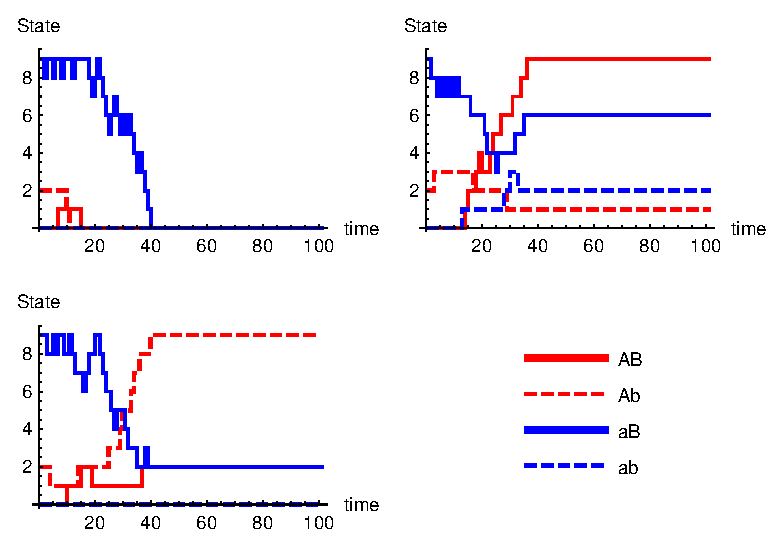
\includegraphics[width=1.0\textwidth]{Figures/gridplot.eps}
\end{frame}

\begin{frame}{$F_A$ from absorbing states}

    The absorbing states $\bold{A} \in \bold{P} \text{ such that } \bold{A}_1,\bold{A}_2 = n \ \text{or } \{0,0,0,0\}$
    
    Process $\bold{X}(t)$.
    
    $P[\bold{X}(\infty) = \bold{A}| \bold{X}(0) = \bold{I}]$ satisfies the left eigenvector with $\lambda = 1$ and a corresponding right eigenvector $=\bold{A}$.
    
    \begin{equation*}
        \vec{p}_\bold{A}^\intercal = \vec{p}_\bold{A}^\intercal \bold{M} \ \ \ \  \text{subject to } p_{\bold{A},\bold{A}}=1 \ \text{and}\ p_{l,\bold{A}}=0
    \end{equation*}
    
    solves for the probabilities to end up in state $\bold{A}$ given initial condition $\bold{I}$.  
    
    \begin{equation*}
    \bold{O}=
        \begin{bmatrix}
        \vec{0}  \\
        \vec{p}_{\bold{A}(1)}  \\
        \vdots  \\
        \vec{p}_{\bold{A}(m)} 
    \end{bmatrix}   
    \end{equation*}
     
    \begin{equation*}
        E[F_A] = (\bold{O} \vec{I}_\bold{I}) \bullet \vec{F}_A   %transpose and do dot product with 
    \end{equation*}
\end{frame}

\begin{frame}{Test frame}
    % Set the overall layout of the tree
\tikzstyle{level 1}=[level distance=3.5cm, sibling distance=3.5cm]
\tikzstyle{level 2}=[level distance=3.5cm, sibling distance=1cm]

% Define styles for bags and leafs
\tikzstyle{bag} = [text width=6em, text centered]
\tikzstyle{end} = [circle, minimum width=3pt,fill, inner sep=0pt]

% The sloped option gives rotated edge labels. Personally
% I find sloped labels a bit difficult to read. Remove the sloped options
% to get horizontal labels. 
\begin{tikzpicture}[grow=right, sloped]
\footnotesize
\node[bag] {$P$}
    child {
        node[bag] {$1-\frac{\sum_i^4 f_i b_i}{\sum_i^4 (f_i b_i + f_i d_i)}$}        
        child {
                node[end, label=right:
                    {$\frac{f_{ab}d_{ab}}{f_{AB} d_{AB}+f_{Ab}d_{Ab}+f_{aB}d_{aB}+f_{ab}d_{ab}}$}] {}
                edge from parent
                node[above] {ab}
                node[below]  {}
            }
            child {
                node[end, label=right:
                    {$\frac{f_{aB}d_{aB}}{f_{AB} d_{AB}+f_{Ab}d_{Ab}+f_{aB}d_{aB}+f_{ab}d_{ab}}$}] {}
                edge from parent
                node[above] {aB}
                node[below]  {}
            }
            child {
                node[end, label=right:
                    {$\frac{f_{Ab}d_{Ab}}{f_{AB} d_{AB}+f_{Ab}d_{Ab}+f_{aB}d_{aB}+f_{ab}d_{ab}}$}] {}
                edge from parent
                node[above] {Ab}
                node[below]  {}
            }
            child {
                node[end, label=right:
                    {$\frac{f_{AB}d_{AB}}{f_{AB} d_{AB}+f_{Ab}d_{Ab}+f_{aB}d_{aB}+f_{ab}d_{ab}}$}] {}
                edge from parent
                node[above] {AB}
                node[below]  {}
            }
            edge from parent 
            node[above] {Death}
            node[below]  {}
    }
    child {
        node[bag] {$\frac{\sum_i^4 f_i b_i}{\sum_i^4 (f_i b_i + f_i d_i)}$}        
        child {
                node[end, label=right:
                    {$f_{ab}-r(f_{AB}f_{ab}-f_{Ab}f_{aB})$}] {}
                edge from parent
                node[above] {ab}
                node[below]  {}
            }
            child {
                node[end, label=right:
                    {$f_{aB}+r(f_{AB}f_{ab}-f_{Ab}f_{aB})$}] {}
                edge from parent
                node[above] {aB}
                node[below]  {}
            }
            child {
                node[end, label=right:
                    {$f_{Ab}+r(f_{AB}f_{ab}-f_{Ab}f_{aB})$}] {}
                edge from parent
                node[above] {Ab}
                node[below]  {}
            }
            child {
                node[end, label=right:
                    {$f_{AB}-r(f_{AB}f_{ab}-f_{Ab}f_{aB})$}] {}
                edge from parent
                node[above] {AB}
                node[below]  {}
            }
        edge from parent         
            node[above] {Birth}
            node[below]  {}
    };
\end{tikzpicture}

\end{frame}

\end{document}